\documentclass[tikz, border=1pt]{standalone}
\usetikzlibrary{fit}
\usepackage{xcolor}
\usetikzlibrary{arrows.meta,decorations.pathreplacing,angles,quotes}

\begin{document}
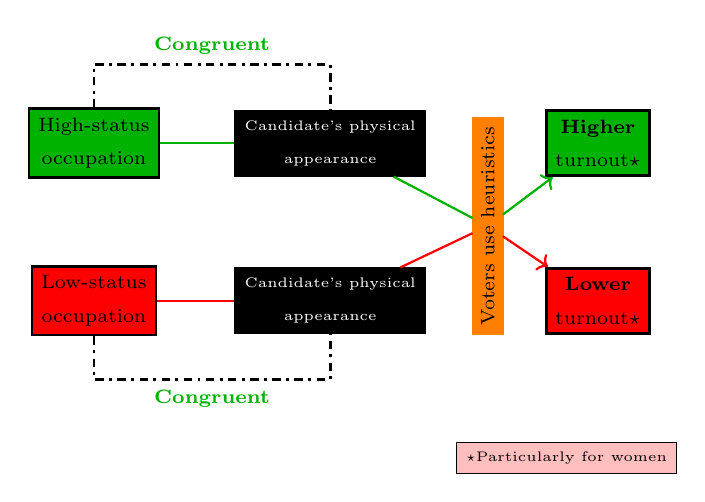
\begin{tikzpicture}[line width=1pt]

% 1
\node[draw,align=center,fill=red,text=black] (B1) at (1,0) {{\scriptsize Low-status}\\{\scriptsize occupation}};
\node[draw,align=center,fill=black,text=white] (B2) at (4,0) {{\tiny Candidate's physical}\\{\tiny appearance}};
%\node[draw,align=center,fill=pink,text=black] (B3) at (6.5,0) {{\scriptsize Female}\\{\scriptsize candidate}};

%\node[draw,align=center,fill=orange,text=black] (B4) at (7,0) {{\tiny Voter uses heuristics}\\{\tiny in low-information}\\{\tiny election}};

\node[draw,fill=red,text=black,align=center] (B5) at (7.4,0) {{\bf {\scriptsize Lower}}\\{\scriptsize turnout$\star$}};


\draw[-,draw=red,thick] (B1) to (B2);
%\draw[-,draw=blue,thick] (B2) to (B4);
%\draw[->,draw=blue,thick] (B3) to (B4);
%\draw[->,draw=blue,thick] (B4) to (B5);



\draw[dash dot] (B1) -- ++(0,-1) -| (B2)
node[below, near start] {{\scriptsize \color{black!30!green}\bf Congruent}};




% 2
\node[draw,align=center,fill=black!30!green,text=black] (A1) at (1,2) {{\scriptsize High-status}\\{\scriptsize occupation}};
\node[draw,align=center,fill=black,text=white] (A2) at (4,2) {{\tiny Candidate's physical}\\{\tiny appearance}};
%\node[draw,,align=center,fill=blue,text=white] (A3) at (6.5,2) {{\scriptsize Male}\\{\scriptsize candidate}};

%\node[draw,,align=center,fill=orange,text=black] (A4) at (7,2) {{\tiny Voter uses heuristics}\\{\tiny in low-information}\\{\tiny election}};

\node[draw,fill=black!30!green,text=black,align=center] (A5) at (7.4,2) {{\bf {\scriptsize Higher}}\\{\scriptsize turnout$\star$}};


\draw[-,draw=black!30!green,thick] (A1) to (A2);
%\draw[-,draw=blue,thick] (A2) to (A4);
%\draw[->,draw=blue,thick] (A3) to (A4);
%\draw[->,draw=blue,thick] (A4) to (A5);



\draw[dash dot] (A1) -- ++(0,1) -| (A2)
node[above, near start] {{\scriptsize \color{black!30!green}\bf Congruent}};




\coordinate (dm1) at (6,2.6);
\coordinate (dm2) at (6,-0.7);
\node[rectangle,minimum width=0.35cm] [fit = (dm1) (dm2)] (bx4) {};
\node[align=center,fill=orange,font=\scriptsize,rotate=90] at (bx4.center) {Voters use heuristics};

\node[draw,fill=pink,font=\tiny,minimum width=0.1cm,thin] at (7,-2) {$\star$Particularly for women};


\draw[-,draw=black!30!green,thick] (A2) to (bx4);
\draw[-,draw=red,thick] (B2) to (bx4);

\draw[->,draw=black!30!green,thick] (bx4) to (A5);
\draw[->,draw=red,thick] (bx4) to (B5);







  
\end{tikzpicture}
\end{document}